\documentclass[hyperref={colorlinks}]{beamer}

\mode<presentation> {\usetheme{default}}

\usepackage{graphicx} % Allows including images
\usepackage{booktabs} % Allows the use of \toprule, \midrule and \bottomrule in tables
\usepackage{algorithm}
\usepackage{algorithmic}
\usepackage{amsmath,amssymb,amsthm}

\newcommand{\set}[1]{\mathbb{#1}}
\newcommand{\trace}[1]{\mathrm{tr}\left(#1\right)}
\newcommand{\rank}[1]{\text{rank}\left(#1\right)}

\algsetup{
	linenosize=\footnotesize,
	linenodelimiter=.
}

%----------------------------------------------------------------------------------------
%	TITLE PAGE
%----------------------------------------------------------------------------------------

\title[ECE 901 Paper Presentation]{Convexified Convolutional Neural Networks} % The short title appears at the bottom of every slide, the full title is only on the title page

\author{Kyle Daruwalla and Akhil Sundararajan}
\institute[UW-Madison]{ECE 901 Fall 2016}
\date{\today}

\begin{document}

\begin{frame}
	\titlepage
\end{frame}

\begin{frame}
	\frametitle{Overview}
	\tableofcontents
\end{frame}

%----------------------------------------------------------------------------------------
%	PRESENTATION SLIDES
%----------------------------------------------------------------------------------------

\section{Background}
\begin{frame}
	\frametitle{Paper Overview}
	\begin{enumerate}
		\item Start generic two-layer CNN
		\item Convex relaxation
		\begin{enumerate}
			\item Linear activation -- optimize for a low-rank matrix $A$ instead of filter weights and coefficients
			\item Non-linear activation -- frame problem in terms of RKHS
		\end{enumerate}
		\item Introduce a kernel-based algorithm for CCNNs
		\item Provide theoretical guarantees on the generalization error
		\item Explain extensions like pooling and multi-layer CNNs
		\item Provide experimental results on MNIST and CIFAR-10
	\end{enumerate}
\end{frame}

\begin{frame}
	\frametitle{Convolutional Neural Networks}
	For an input vector, $x \in \set{R}^{d_0}$, and output vector, $y \in \set{R}^{d_2}$, define
	$$\{z_p(x) \mid z_p(x) \in \set{R}^{d_1}\}_{j = 1}^P$$
	to be the set of $P$ patches of $x$. \\
	For a given $\sigma: \set{R} \mapsto \set{R}$, the output of a filter is
	$$h_j(z) = \sigma(w_j^T z)$$
	The output of a CNN is $f = (f_1(x), f_2(x), \ldots, f_{d_2}(x))$ is defined as
	\begin{equation}
		f_k(x) = \sum_{j = 1}^r \sum_{p = 1}^P \alpha_{k, j, p} h_j(z_p(x))
		\label{eq:cnn-output}
	\end{equation}
\end{frame}

\begin{frame}
	\frametitle{Convolutional Neural Networks}
	CNNs are described by the class of models:
	\begin{align}
		\mathcal{F}_{\text{cnn}}(B_1, B_2) = \{f \text{ of the form Eq. \ref{eq:cnn-output} } & \mid \max_{j \in [r]} \|w_j\|_2 \leq B_1 \\ \nonumber
		\text{ and } & \max_{k \in [d_2], j \in [r]} \|\alpha_{k, j}\|_2 \leq B_2\}
		\label{eq:fcnn-class}
	\end{align}
	Given a set of samples $\{(x_i, y_i)\}_{i = 1}^n$, we want to solve the ERM:
	\begin{equation}
		\hat{f}_{\text{cnn}} = \arg \min_{f \in \mathcal{F}_{\text{cnn}}} \sum_{i = 1}^n \mathcal{L}(f(x_i), y_i)
		\label{eq:cnn-erm}
	\end{equation}
\end{frame}

\section{Convex Relaxations}
\subsection{Linear Activation Functions}
\begin{frame}
	\frametitle{Optimizing For Low-Rank Matrix (Linear Activation)}
	For $x \in \set{R}^{d_0}$, define
	$$Z(x) = \left[\begin{matrix}
		z_1(x)^T \\
		\vdots \\
		z_P(x)^T
	\end{matrix}\right] \text{ and } \alpha_{k, j} = \left[\begin{matrix}
		\alpha_{k, j, 1} \\
		\vdots \\
		\alpha_{k, j, P}
	\end{matrix}\right]$$
	Then rewrite Eq. \ref{eq:cnn-output} with activation function, $\sigma(t) = t$, as
	\begin{equation}
		f_k(x) = \sum_{j = 1}^r \alpha_{k, j}^T Z(x) w_j = \trace{Z(x) \sum_{j = 1}^r w_j \alpha_{k, j}^T} = \trace{Z(x) A_k}
		\label{eq:cnn-output-modified}
	\end{equation}
\end{frame}

\begin{frame}
	\frametitle{Optimizing For Low-Rank Matrix (Linear Activation)}
	\begin{figure}
		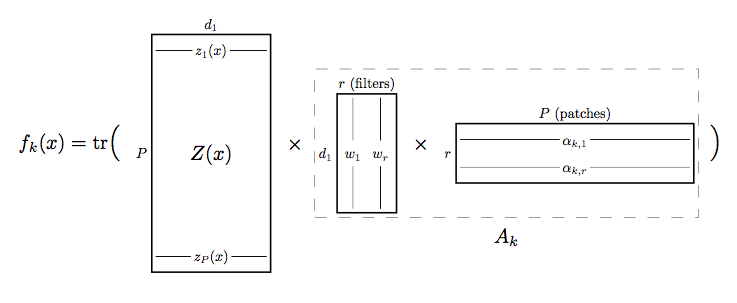
\includegraphics[scale=0.3]{Linear-Case-Structure.png}
		\caption{Reframing the problem in terms of a low-rank matrix, $A_k$, allows for convex optimization over a nuclear norm ball}
		\label{fig:linear-case-structure}
	\end{figure}
\end{frame}

\begin{frame}
	\frametitle{Optimizing For Low-Rank Matrix (Linear Activation)}
	The CNN class of models is then
	\begin{align}
		\mathcal{F}_{\text{cnn}}(B_1, B_2) = \{f \text{ of the form Eq. \ref{eq:cnn-output-modified} } & \mid \max_{j \in [r]} \|w_j\|_2 \leq B_1 \\ \nonumber
		\text{ and } & \max_{k \in [d_2], j \in [r]} \|\alpha_{k, j}\|_2 \leq B_2\} \\ \nonumber
		\text{ and } & \rank{A} = r
		\label{eq:fcnn-class-modified}
	\end{align}
	Define the CCNN class of models as
	\begin{equation}
		\mathcal{F}_{\text{ccnn}}(B_1, B_2) = \{f \text{ of the form Eq. \ref{eq:cnn-output-modified} } \mid \|A\|_* \leq B_1 B_2 r \sqrt{d_2}\}
		\label{eq:fccnn-class}
	\end{equation}
	where $\mathcal{F}_{\text{cnn}}(B_1, B_2) \subseteq \mathcal{F}_{\text{ccnn}}(B_1, B_2)$.
\end{frame}

\subsection{Non-Linear Activation Functions}
\begin{frame}
	\frametitle{Reproducing Kernel Hilbert Space (RKHS)}
	\begin{itemize}
		\item 	Hilbert Space: a complete inner-product space
		\item 	a reproducing kernel Hilbert space is
		\begin{itemize}
			\item a Hilbert space of functions $f: \mathcal{X}\rightarrow \mathbb{R}$
			\item evaluation functionals are continuous
		\end{itemize}
	\item reproducing kernel (associated with Hilbert Space $\mathcal{H}$): a function $\mathcal{K}: \mathcal{X}\times\mathcal{X}\rightarrow\mathbb{R}$ such that
	\begin{itemize}
		\item $\mathcal{K}(x,\cdot)=\mathcal{K}_x(\cdot)\in\mathcal{H}, \forall x\in \mathcal{X}$
		\item $\langle f,\mathcal{K}_x \rangle_{\mathcal{H}} = f(x), \forall f\in\mathcal{H}$ (reproducing property)
	\end{itemize}
	\item
	\begin{itemize}
		\item $\mathcal{H}$ is an RKHS $\implies$ $\exists$ unique reproducing kernel $\mathcal{K}$
		\item If $\exists$ reproducing kernel $\mathcal{K}$ $\implies$ $\mathcal{H}$ is an RKHS 
	\end{itemize}
	\end{itemize}
\end{frame}


\begin{frame}
	\frametitle{Framing Problem Using RKHS}
	\begin{itemize}
		\item for certain kernels $\mathcal{K}$ and activations $\sigma$, Representer Theorem implies that for any patch $z_p(x_i)$
		\begin{align*}
			h(z_p(x_i))=\sum\limits_{(i',p')\in[n]\times[p]} c_{i',p'}k(z_p(x_i),z_{p'}(x_{i'}))
		\end{align*}
		\item choose kernel matrix $K=\mathbb{R}^{nP\times nP}$
		\item consider $K=QQ^{\top}$
		\begin{align*}
			h(z_p(x_i))=\langle Q_{(i,p)},w \rangle \text{ where } w:=\sum\limits_{(i',p')} c_{(i',p')}Q_{(i',p')}
		\end{align*}
	\end{itemize}
\end{frame}

\section{Algorithm}
\begin{frame}
	\frametitle{CCNN Algorithm}
	~
	\begin{algorithm}[H]
		\caption{CCNN Algorithm}
		\label{alg:ccnn-algorithm}
		\footnotesize
		\begin{algorithmic}[1]
			\REQUIRE Data $\{(x_i, y_i)\}_{i = 1}^n$, kernel function $\mathcal{K}$, regularization parameter $R > 0$, number of filters $r$
			\STATE Construct a matrix $K \in \set{R}^{nP \times nP}$ such that the entry at column $(i, p)$ and row $(i', p')$ is $\mathcal{K}(z_p(x_i), z_{p'}(x_{i'})$. Compute the factorization $K = QQ^T$ or an approximation, $K \approx QQ^T$, where $Q \in \set{R}^{nP \times m}$.
			\STATE For each $x_i$, construct a patch matrix $Z(x_i) \in \set{R}^{P \times m}$ whose $p$-th row is the $(i, p)$-th row of $Q$.
			\STATE Solve the following optimization problem to obtain a matrix $\hat{A} = (\hat{A}_1, \ldots, \hat{A}_{d_2})$
			$$\hat{A} = \arg \min_{\|A\|_* \leq R} \tilde{\mathcal{L}}(A) \text{ where } \tilde{\mathcal{L}}(A) = \sum_{i = 1}^n \mathcal{L}\left((\trace{Z(x_i) A_1}, \ldots, \trace{Z(x_i) A_{d_2}}), y_i\right)$$
			\STATE Compute a rank-$r$ approximation $\tilde{A} \approx \hat{U} \hat{V}^T$ where $\hat{U} \in \set{R}^{m \times r}$ and $\hat{V} \in \set{R}^{Pd_2 \times r}$.
			\RETURN The predictor $\hat{f}_{\text{ccnn}}(x) = \left(\trace{Z(x) \hat{A}_1}, \ldots, \trace{Z(x) \hat{A}^{d_2}}\right)$ and the convolutional layer output $H(x) = \hat{U}^T (Z(x))^T$.
		\end{algorithmic}
	\end{algorithm}
\end{frame}

\begin{frame}
	\frametitle{Solving ERM in CCNN Algorithm}
	\begin{itemize}
		\item projected gradient descent
		\begin{align*}
			A^{t+1}=\Pi_R(A^t-\eta^t\nabla_A\tilde{\mathcal{L}}(A^t))
		\end{align*}
		\item compute SVD of $A$, the project singular values onto $l_1$ ball (Duchi et al)
		\item proximal adaptive gradient method
		\item proximal SVRG
	\end{itemize}
\end{frame}

\section{Theoretical Results}
\begin{frame}
	\frametitle{Choice of Kernel}
	\begin{itemize}
		\item kernel functions considered must satisfy notion of richness
		\begin{align*}
			&\mathcal{K}(z,z')=\frac{1}{2-\langle z,z' \rangle}, \hspace{4mm} ||z||_2\leq 1, ||z'||_2\leq 1 \\
			&\mathcal{K}(z,z')=exp(-\gamma||z-z'||_2^2), \hspace{4mm} |z||_2=||z'||_2 =1, \gamma\geq0
		\end{align*}
	\end{itemize}
\end{frame}
\begin{frame}
	\frametitle{Valid Activation Functions}
	\begin{itemize}
		\item arbitrary polynomial functions
		\item $\sigma(t)=\sin(t)$
		\item $\sigma_{erf}(t)=\frac{2}{\sqrt{pi}}\int_{0}^{t}e^{-z^2}dz$
		\item $\sigma_{sh}(t)=\frac{1}{2}\int_{-\infty}^{t}(\sigma_{erf}(z)+1)dz$
	\end{itemize}
	\begin{figure}
		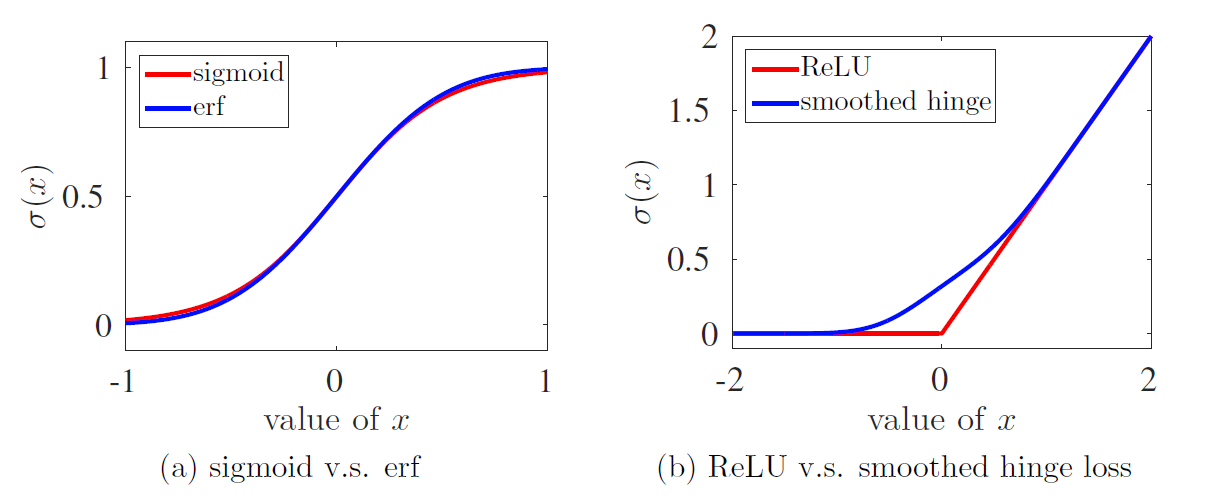
\includegraphics[scale=0.4]{Valid-Activation.png}
		\caption{approximations to activations which are not smooth enough}
		\label{fig:valid-activation}
	\end{figure}
\end{frame}
\begin{frame}
	\frametitle{Theorem 1: Bound on Generalization Error}
		\begin{itemize}
			\item loss function $\mathcal{L}(;y)$ is L-Lipschitz continuous for every $y \in [d_2]$
			\item $\mathcal{K}$ is the inverse polynomial kernel or the Gaussian RBF kernel
			\item valid activation function $\sigma$
			\item $c>0$
			\item radius $R:=C_\sigma(B_1)B_2r$
		\end{itemize}
	\begin{align*}
		&\exists C_\sigma(B_1) \text{ such that } \\
		&\mathbb{E}_{X,Y}[\mathcal{L}(\hat{f}_{ccnn}(X);Y)]\leq \\ 
		&\inf\limits_{f\in \mathcal{F}_{cnn}} \mathbb{E}_{X,Y}[\mathcal{L}(f(X);Y)]+ \frac{cLC_{\sigma}(B_1)B_2 r\sqrt{log(nP)\mathbb{E}_X[||K(X)||_2]}}{\sqrt{n}}
	\end{align*}	
\end{frame}

\begin{frame}
	\frametitle{Proof Sketch}
	\begin{enumerate}
		\item consider a relaxed function class
		\begin{align*}
			\mathcal{F}_{ccnn}:=\Big\{x\mapsto \sum_{j = 1}^{r^*} \sum_{p = 1}^P \alpha_{j, p} h_j(z_p(x)) : r^*<\infty \\ 
			\text{ and } \sum_{j = 1}^{r^*} ||\alpha_j||_2||h_j||_{\mathcal{H}}\leq C_{\sigma}(B_1)B_2d_2 \Big\}
		\end{align*}
		\item characterize Rademacher complexity of $\mathcal{F}_{ccnn}$ to upper bound generalization error of $\hat{f}_{ccnn}$
	\end{enumerate}
\end{frame}

\begin{frame}
	\frametitle{Further Proof Details (1/4)}
	Lemma 1:
	\begin{align*}
		\text{For any valid } \sigma(\cdot), \text{ } \exists C_{\sigma}(B_1) \text{ s.t. } \mathcal{F}_{cnn}\subset\mathcal{F}_{ccnn}
	\end{align*}
	Lemma 4:
	\begin{align*}
		&\text{With CCNN hyper-parameter } R=C_\sigma(B_1)B_2d_2, \\
		&\hat{f}_{ccnn} \text{ is guaranteed to satisfy } \hat{f}_{ccnn} \in \arg\min\limits_{f\in\mathcal{F}_{ccnn}} \sum\limits_{i=1}^{n} \mathcal{L}(f(x_i);y_i)
	\end{align*}
\end{frame}

\begin{frame}
	\frametitle{Further Proof Details (2/4)}
	the Rademacher complexity of $\mathcal{F}=\{f:\mathcal{X}\rightarrow \mathbb{R}\}$ with respect to $n$ i.i.d. samples $\{X_i\}_{i=1}^n$ is given by
	\begin{align*}
	\mathcal{R}_n(\mathcal{F}):=\mathbb{E}_{X,\epsilon} \bigg[\sup\limits_{f\in\mathcal{F}} \frac{1}{n}\sum\limits_{i=1}^n \epsilon_i f(X_i)\bigg]
	\end{align*}
	where $\{\epsilon_i\}_{i=1}^n$ are an i.i.d. sequence of uniform $\{-1,+1\}$-valued random variables
\end{frame}

\begin{frame}
	\frametitle{Further Proof Details (3/4)}
	Lemma 5: \\
	$\exists$ universal constant $c$ such that 
	\begin{align*}
		\mathcal{R}_n(\mathcal{F}_{ccnn})\leq \frac{cC_{\sigma}(B_1)B_2r\sqrt{log(nP)\mathbb{E}[||K(X)||_2]}}{\sqrt{n}}
	\end{align*}
	generalization bound:
	\begin{align*}
		\mathbb{E}[\mathcal{L}(\mathcal{F}_{ccnn}(X);Y)]\leq \inf\limits_{f\in \mathcal{F}_{ccnn}} \mathbb{E}[\mathcal{L}(f(x);y)]+2L\mathcal{R}_n(\mathcal{F}_{ccnn})+\frac{c}{\sqrt{n}}
	\end{align*}
\end{frame}

\begin{frame}
	\frametitle{Further Proof Details (4/4)}
	By Lemma 3,
	\begin{align*}
	\inf\limits_{f\in \mathcal{F}_{ccnn}} \mathbb{E}[\mathcal{L}(f(x);y)] \leq \inf\limits_{f\in \mathcal{F}_{cnn}} \mathbb{E}[\mathcal{L}(f(x);y)]
	\end{align*}
	It follows that
	\begin{align*}
	\mathbb{E}_{X,Y}[\mathcal{L}(\hat{f}_{ccnn}(X);Y)]\leq 
	&\inf\limits_{f\in \mathcal{F}_{cnn}} \mathbb{E}_{X,Y}[\mathcal{L}(f(X);Y)]+ \\ &\frac{cLC_{\sigma}(B_1)B_2 r\sqrt{log(nP)\mathbb{E}_X[||K(X)||_2]}}{\sqrt{n}}
	\end{align*}
\end{frame}

\section{Experimental Results}
\begin{frame}
	\frametitle{Experimental Results}
	On MNIST dataset:
	\begin{table}
		\begin{tabular}{|l|c|c|c|c|c|}
			\hline
			 & \texttt{basic} & \texttt{rand} & \texttt{rot} & \texttt{img} & \texttt{img+rot} \\
			\hline
			SVM$_{rbf}$ & 3.03\% & 14.58\% & \textbf{11.11\%} & 22.61\% & 55.18\% \\
			NN-1 & 4.69\% & 20.04\% & 18.11\% & 27.41\% & 62.16\% \\
			CNN-1 (ReLU) & 3.37\% & 9.83\% & 18.84\% & 14.23\% & 45.96\% \\
			CCNN-1 & \textbf{2.38\%} & \textbf{7.45\%} & 13.39\% & \textbf{10.40\%} & \textbf{42.28\%} \\
			\hline
			TIRBM & - & - & \textbf{4.20\%} & - & 35.50\% \\
			SDAE-3 & 2.84\% & 10.30\% & 9.53\% & 16.68\% & 43.76\% \\
			ScatNet-2 & 1.27\% & 12.30\% & 7.48\% & 18.40\% & 50.48\% \\
			PCANet-2 & \textbf{1.06\%} & 6.19\% & 7.37\% & 10.95\% & 35.48\% \\
			CNN-2 (ReLU) & 2.11\% & 5.64\% & 8.27\% & 10.17\% & 32.42\% \\
			CNN-2 (Quad) & 1.75\% & 5.30\% & 8.83\% & 11.60\% & 36.90\% \\
			CCNN-2 & 1.38\% & \textbf{4.32\%} & 6.98\% & \textbf{7.46\%} & \textbf{30.23\%} \\
			\hline
		\end{tabular}
		\caption{Classification error with a Gaussian kernel for CCNNs}
		\label{tab:mnist-results}
	\end{table}
\end{frame}

\begin{frame}
	\frametitle{Experimental Results}
	On CIFAR-10 dataset:
	\begin{table}
		\begin{tabular}{|l|c|}
			\hline
			 & Error Rate \\
			\hline
			CNN-1 & 34.14\% \\
			CCNN-1 & \textbf{23.62\%} \\
			\hline
			CNN-2 & 24.98\% \\
			CCNN-2 & \textbf{20.52\%} \\
			\hline
			SVM$_{Fastfood}$ & 36.90\% \\
			PCANet-2 & 22.86\% \\
			CKN & 21.70\% \\
			CNN-3 & 21.48\% \\
			CCNN-3 & \textbf{19.56\%} \\
			\hline
		\end{tabular}
		\caption{Error rate with a Gaussian kernel for CCNNs}
		\label{tab:cifar-10-results}
	\end{table}
\end{frame}

%------------------------------------------------

\begin{frame}
	\frametitle{References}
	\footnotesize{
		\begin{thebibliography}{9} % Beamer does not support BibTeX so references must be inserted manually as below
			\bibitem[Zhang, 2016]{zhang2016}
			Y. Zhang, et al. (2016, Sept. 4).
			\emph{Convexified Convolutional Neural Networks} (v1) [Online].
			Available: \url{https://arxiv.org/abs/1609.01000}
		\end{thebibliography}
	}
\end{frame}

%------------------------------------------------

\begin{frame}
	\Huge{\centerline{The End}}
\end{frame}

\end{document} 